% mostra conceitos sobre bibtex em geral

\documentclass{article}

\usepackage[utf8]{inputenc}
\usepackage{graphicx}
\usepackage[brazil]{babel}

\begin{document}
	\section{Introdução}
		Documento exemplo para consultas futuras do \LaTeX.

	\section{Acentuação}		
		Ele será incrementado a cada etapa nesse minicurso super legal.
	
	\section{Negrito, Itálico, Ê1nfase}
		A codificação no \textbf{Linux} deve \huge sempre \normalsize ser utilizada em \textbf{UTF-8} para acentuação \emph{correta}. No \textit{Windows} a \emph{maioria} dos casos utiliza-se o \textit{Latin1}.
		
	\section{\textit{Environment}}
		Nesta seção mostram-se alguns ambientes disponíveis para uso no \LaTeX. Por exemplo na subseção \ref{verbatim} o ambiente \textsf{verbatim} não interpretará inserido.

		\subsection{\textit{Enumerate}}
			\begin{enumerate}
				\item	O \LaTeX provê uma forma diferente para numeração;
				\item	Como sempre focamos no conteúdo, não na formatação;
				\item[A.]	Podemos usar outra letra também.
			\end{enumerate}
	
		\subsection{\textit{Itemize}}
			Só mudamos uma palavra para transformar o texto:
			\begin{itemize}
				\item	O \LaTeX provê uma forma diferente para numeração;
				\item	Como sempre focamos no conteúdo, não na formatação;
				\item[A.]	Podemos usar outra letra também.
			\end{itemize}
	
		\subsection{\textit{Description}}
			Algumas siglas citadas na apresentação:
			\begin{description}
				\item[ACM] \textit{Association for Computing Machinery}
				\item[IEEE]	\textit{Institute of Electrical and Electronic Engineers}
				\item[SBC] Sociedade Brasileira da Computação
			\end{description}

		\subsection{\textit{Verbatim}}
			\label{verbatim}\verb|\textbf{Porquê esse texto não fica em negrito?}|
	
	\section{Figuras}
		% Falar sobre environment;
		% Tradeoff entre caption e environment
		% Pacote {babel}
		\begin{figure}[h]
			\centering
			\label{pinto}
			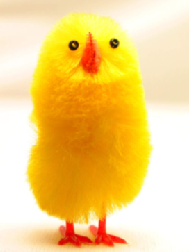
\includegraphics{chick.png}
			\caption{O pintinho amarelinho}
		\end{figure}
	
	\section{Tabela}
		\begin{table}[h]
			\centering
			\begin{tabular}{c|c}
				\hline	Cabecalho1			&	Cabecalho2	\\
				\hline	Conteudo coluna 1	&	Conteudo Coluna 2	\\
				\hline	Conteudo coluna 1	&	Conteudo Coluna 2	\\
				\hline	Conteudo coluna 1	&	Conteudo Coluna 2	\\
				\hline
			\end{tabular}
			\caption{Pequena tabela de exemplo}
		\end{table}
	
	\section{Referências}
		A maneira mais eficaz de fazer referências no \LaTeXe é utilizar um arquivo principal de referências \textsf{.bib}, editá-lo com o \textsf{JabRef} e incluí-lo no \textsf{.tex} com \newline\verb|\bibliography{nome_do_.bib}|. 
		
		Normalmente, precisa-se também indicar a formatação dos estilos por \verb|\bibliographystyle{Algum_Tipo}|.

		
\nocite{Knuth:1997:ACP:260999,Knuth:1997:ACP:270146,Knuth:1998:ACP:280635}
\bibliographystyle{plain}
\bibliography{referencias}
\end{document}